% Reference https://www.youtube.com/watch?v=Boltwen-g1g&ab_channel=ChandraHas
%DIF LATEXDIFF DIFFERENCE FILE
%DIF DEL ./before_peer_review/supp.tex   Wed Nov  3 11:32:05 2021
%DIF ADD ./rev_2/supp.tex                Mon Dec 20 14:56:46 2021

\documentclass[11pt,a4paper]{article}

% General
\usepackage[margin=1in]{geometry}
\usepackage[sort&compress,square,numbers]{natbib}
\usepackage{amsmath}
\usepackage{lipsum,times,graphicx,hyperref,cleveref}
\hypersetup{nolinks=true}
\usepackage[labelfont=bf]{caption}
\usepackage{amssymb}

\usepackage{physics}
\usepackage{siunitx}
\usepackage{listings}
%DIF 17a17
\usepackage{array,multirow} %DIF > 
%DIF -------

% More graphics
\usepackage[label font={bf, normalsize}]{subfig}
\renewcommand{\thesubfigure}{\Alph{subfigure}}
\usepackage{caption}
\captionsetup{font=normal}
\usepackage{floatrow}
\floatsetup[figure]{subcapbesideposition=top}
\floatsetup[table]{style=plaintop}

\usepackage{titling}
\renewcommand\maketitlehooka{\null\mbox{}\vfill}
\renewcommand\maketitlehookd{\vfill\null}

%DIF 32a33-36
\usepackage{xr} %DIF > 
\externaldocument[main-]{main} %DIF > 
\externaldocument[fig-]{figures} %DIF > 
 %DIF > 
%DIF -------
\title{\vspace{-5cm} {Supplementary material}\\[5mm] 
\textbf{Behavior of weakly adsorbing protein impurities in flow-through ion-exchange chromatography}}
% \DIFdelbegin \DIFdel{\textbf{Behavior of weakly adsorbing impurities in flow-through ion-exchange chromatography}}\DIFdelend \DIFaddbegin \DIFadd{\textbf{Behavior of weakly adsorbing protein impurities in flow-through ion-exchange chromatography}}\DIFaddend }
 
\author{Chase E. Herman, Xuankuo Xu, Steven J. Traylor, Sanchayita Ghose, \and Zheng Jian Li, and Abraham M. Lenhoff}

\date{}
%DIF 38a43-44
 %DIF > 
%DIF -------

%\renewcommand{\figurename}{Fig.}
\renewcommand{\baselinestretch}{1.33} 
\renewcommand{\thepage}{S\arabic{page}}
\renewcommand{\thetable}{S\arabic{table}}
\renewcommand{\thefigure}{S\arabic{figure}}
\renewcommand{\theequation}{S\arabic{equation}}
%==============================Content=========================
%DIF PREAMBLE EXTENSION ADDED BY LATEXDIFF
%DIF UNDERLINE PREAMBLE %DIF PREAMBLE
\RequirePackage[normalem]{ulem} %DIF PREAMBLE
\RequirePackage{color}\definecolor{RED}{rgb}{1,0,0}\definecolor{BLUE}{rgb}{0,0,1} %DIF PREAMBLE
\providecommand{\DIFaddtex}[1]{{\protect\color{blue}\uwave{#1}}} %DIF PREAMBLE
\providecommand{\DIFdeltex}[1]{{\protect\color{red}\sout{#1}}}                      %DIF PREAMBLE
%DIF SAFE PREAMBLE %DIF PREAMBLE
\providecommand{\DIFaddbegin}{} %DIF PREAMBLE
\providecommand{\DIFaddend}{} %DIF PREAMBLE
\providecommand{\DIFdelbegin}{} %DIF PREAMBLE
\providecommand{\DIFdelend}{} %DIF PREAMBLE
\providecommand{\DIFmodbegin}{} %DIF PREAMBLE
\providecommand{\DIFmodend}{} %DIF PREAMBLE
%DIF FLOATSAFE PREAMBLE %DIF PREAMBLE
\providecommand{\DIFaddFL}[1]{\DIFadd{#1}} %DIF PREAMBLE
\providecommand{\DIFdelFL}[1]{\DIFdel{#1}} %DIF PREAMBLE
\providecommand{\DIFaddbeginFL}{} %DIF PREAMBLE
\providecommand{\DIFaddendFL}{} %DIF PREAMBLE
\providecommand{\DIFdelbeginFL}{} %DIF PREAMBLE
\providecommand{\DIFdelendFL}{} %DIF PREAMBLE
%DIF HYPERREF PREAMBLE %DIF PREAMBLE
\providecommand{\DIFadd}[1]{\texorpdfstring{\DIFaddtex{#1}}{#1}} %DIF PREAMBLE
\providecommand{\DIFdel}[1]{\texorpdfstring{\DIFdeltex{#1}}{}} %DIF PREAMBLE
%DIF LISTINGS PREAMBLE %DIF PREAMBLE
\RequirePackage{listings} %DIF PREAMBLE
\RequirePackage{color} %DIF PREAMBLE
\lstdefinelanguage{DIFcode}{ %DIF PREAMBLE
%DIF DIFCODE_UNDERLINE %DIF PREAMBLE
  moredelim=[il][\color{red}\sout]{\%DIF\ <\ }, %DIF PREAMBLE
  moredelim=[il][\color{blue}\uwave]{\%DIF\ >\ } %DIF PREAMBLE
} %DIF PREAMBLE
\lstdefinestyle{DIFverbatimstyle}{ %DIF PREAMBLE
	language=DIFcode, %DIF PREAMBLE
	basicstyle=\ttfamily, %DIF PREAMBLE
	columns=fullflexible, %DIF PREAMBLE
	keepspaces=true %DIF PREAMBLE
} %DIF PREAMBLE
\lstnewenvironment{DIFverbatim}{\lstset{style=DIFverbatimstyle}}{} %DIF PREAMBLE
\lstnewenvironment{DIFverbatim*}{\lstset{style=DIFverbatimstyle,showspaces=true}}{} %DIF PREAMBLE
%DIF END PREAMBLE EXTENSION ADDED BY LATEXDIFF

\begin{document}

\begin{titlingpage}
\maketitle
\end{titlingpage}

\begin{figure}[H]
    \centering
    \DIFdelbeginFL %DIFDELCMD < \sidesubfloat[]{\includegraphics[width=0.75\textwidth]%
%DIFDELCMD <                     {breakthrough_curves_c_1000_ug_ml}\label{sfig:1 mg/ml}}
%DIFDELCMD <     %%%
\DIFdelendFL \DIFaddbeginFL \sidesubfloat[]{\includegraphics[width=0.75\textwidth]%
                    {figure_s1a}\label{sfig:1 mg/ml}}
    \DIFaddendFL \\
    \DIFdelbeginFL %DIFDELCMD < \sidesubfloat[]{\includegraphics[width=0.75\textwidth]%
%DIFDELCMD <                     {breakthrough_curves_c_100_ug_ml}\label{sfig:100 ug/ml}}
%DIFDELCMD <     %%%
\DIFdelendFL \DIFaddbeginFL \sidesubfloat[]{\includegraphics[width=0.75\textwidth]%
                    {figure_s1b}\label{sfig:100 ug/ml}}
    \DIFaddendFL \\
    \DIFdelbeginFL %DIFDELCMD < \sidesubfloat[]{\includegraphics[width=0.75\textwidth]%
%DIFDELCMD <                     {breakthrough_curves_c_10_ug_ml}\label{sfig:10 ug/ml}}
%DIFDELCMD <     %%%
\DIFdelendFL \DIFaddbeginFL \sidesubfloat[]{\includegraphics[width=0.75\textwidth]%
                    {figure_s1c}\label{sfig:10 ug/ml}}
    \DIFaddendFL 

    \caption{Breakthrough profiles from a simulation of solute loading at \protect\subref{sfig:1 mg/ml} 1 mg/ml, \protect\subref{sfig:100 ug/ml} 100 $\mu$g/ml, and \protect\subref{sfig:10 ug/ml} 10 $\mu$g/ml. Lines correspond to simulations with different $K_{eq}$, which increases by 4 orders of magnitude from left to right. Note that $q_{max}$ was fixed at 100 mg/ml of packed column for all simulations, and the abscissa is on a logarithmic scale.} 

    \label{fig:exploratory breakthrough curves - other concentrations}
\end{figure}

\begin{figure}[H]
    \centering
    \vspace{-5.2cm}
    \makebox[\textwidth][c]{\DIFdelbeginFL %DIFDELCMD < 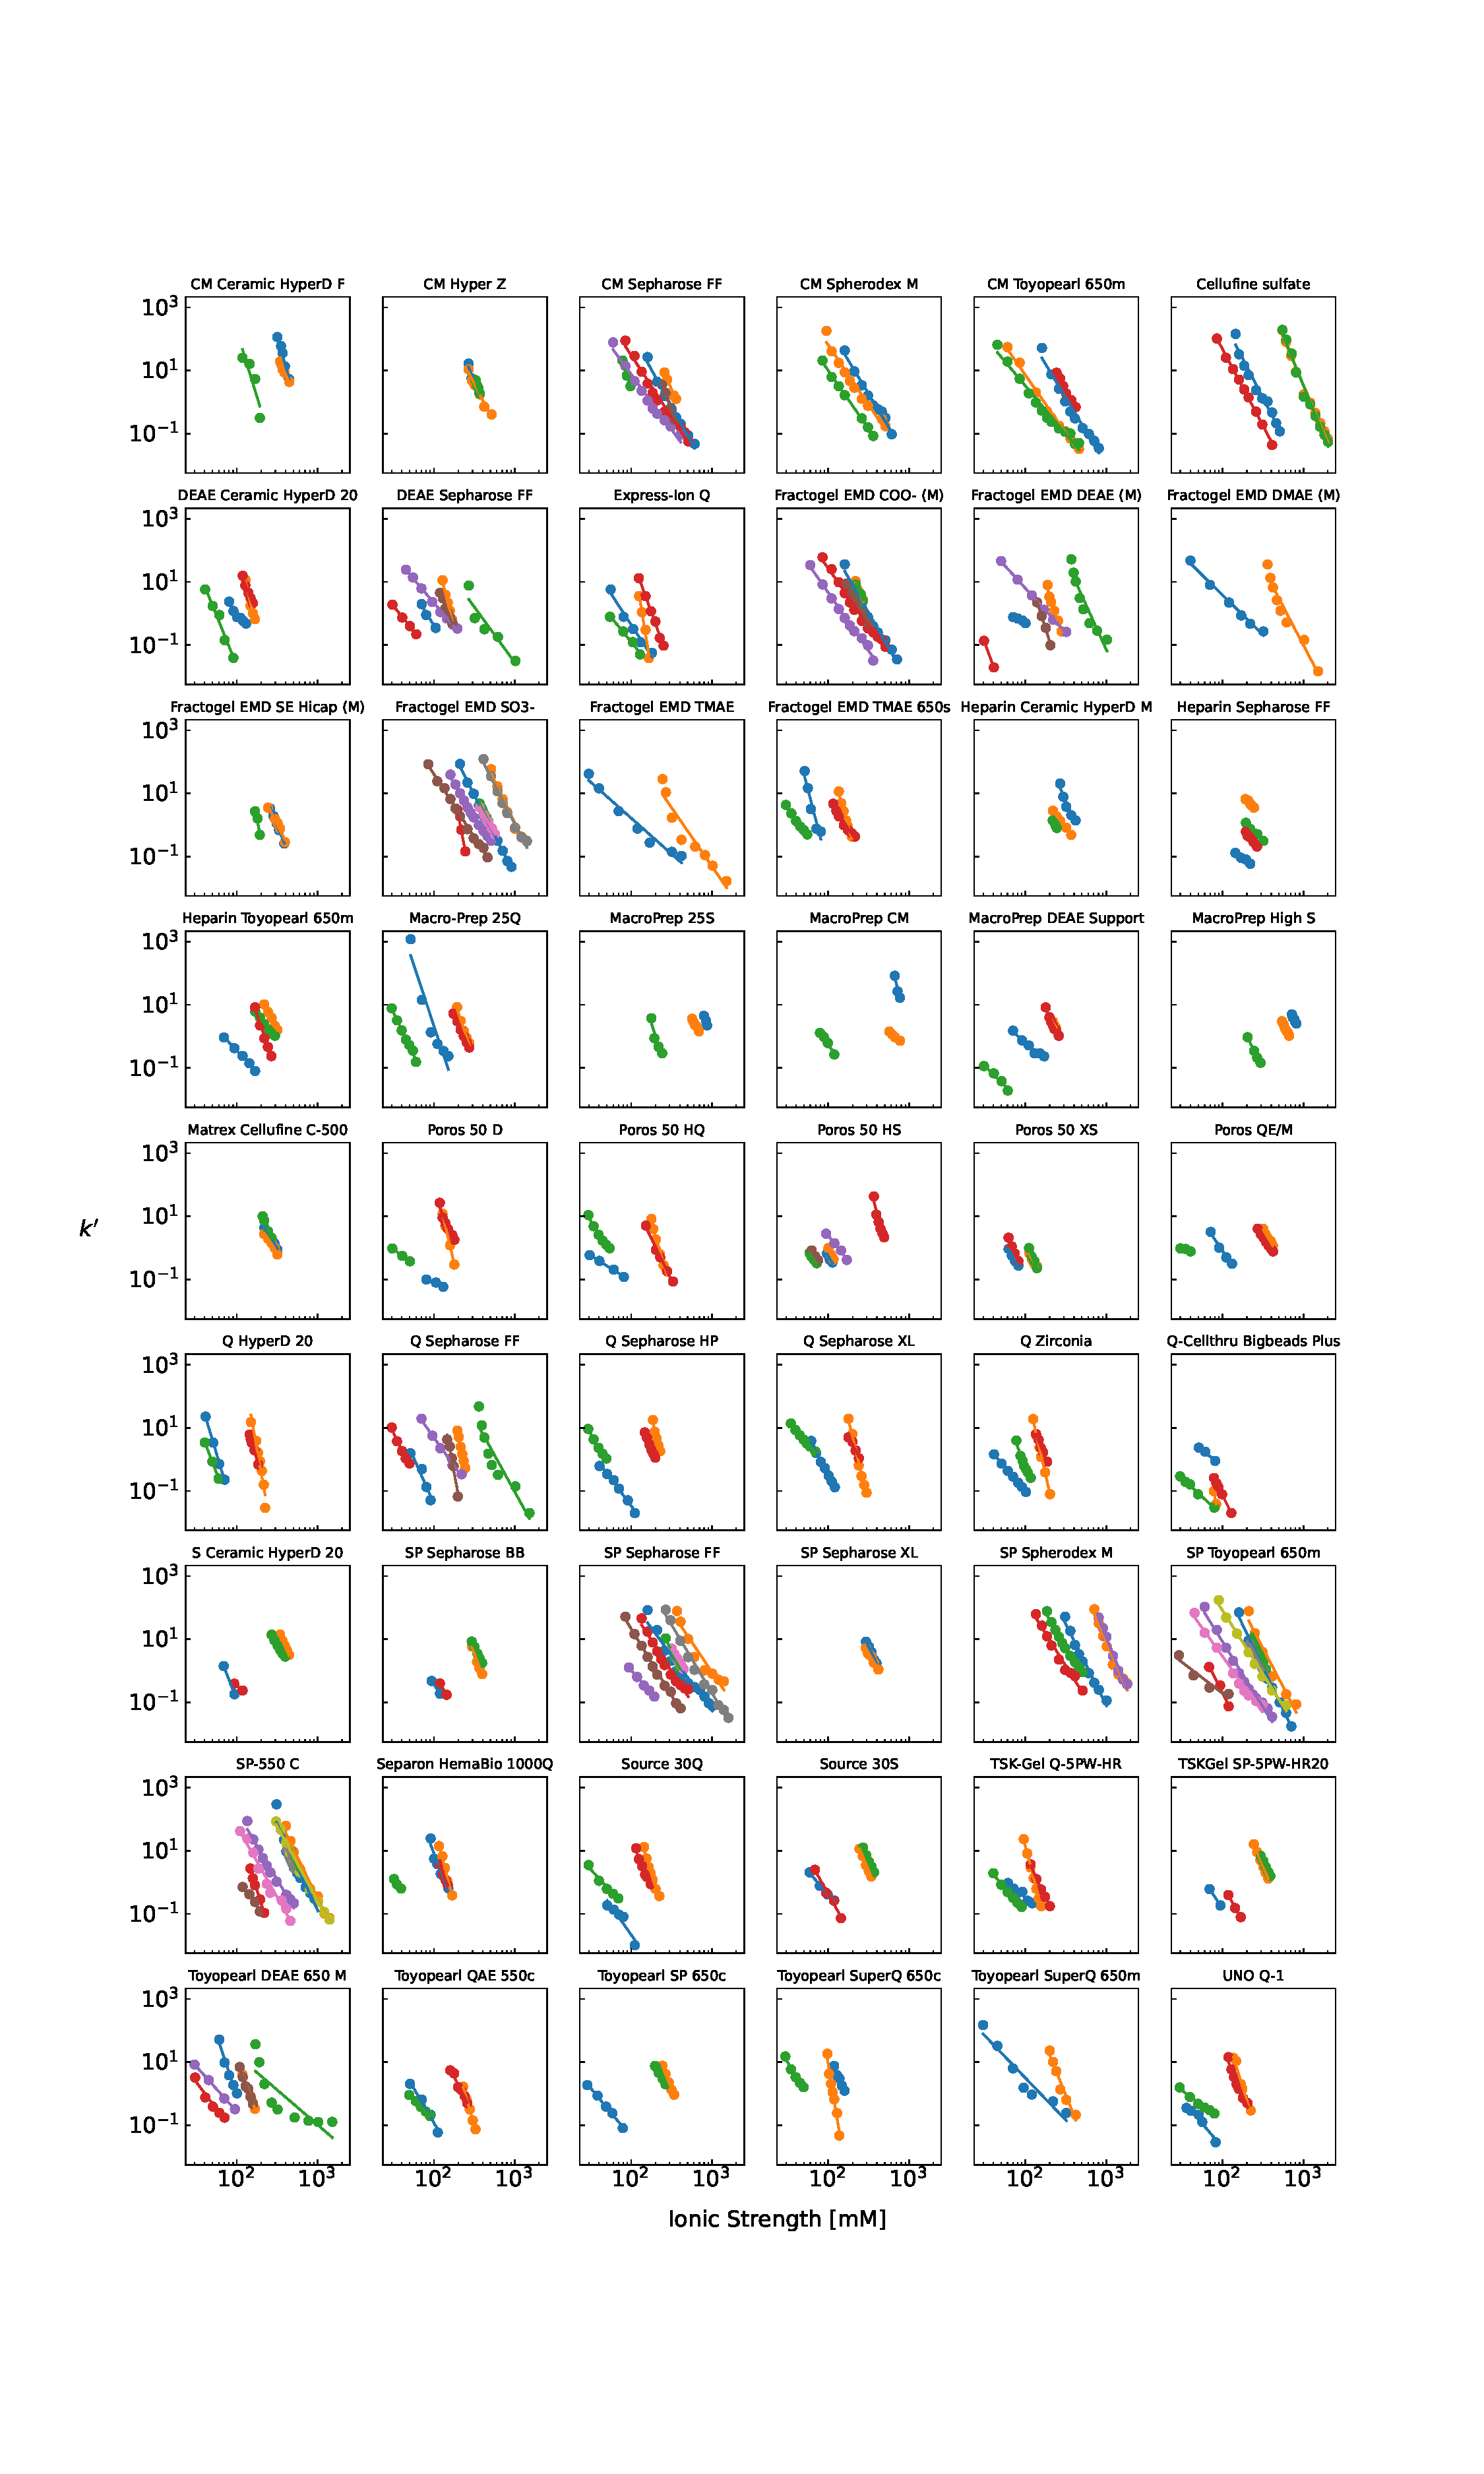
\includegraphics[width=1.2\textwidth]{lit_kprime_data}%%%
\DIFdelendFL \DIFaddbeginFL 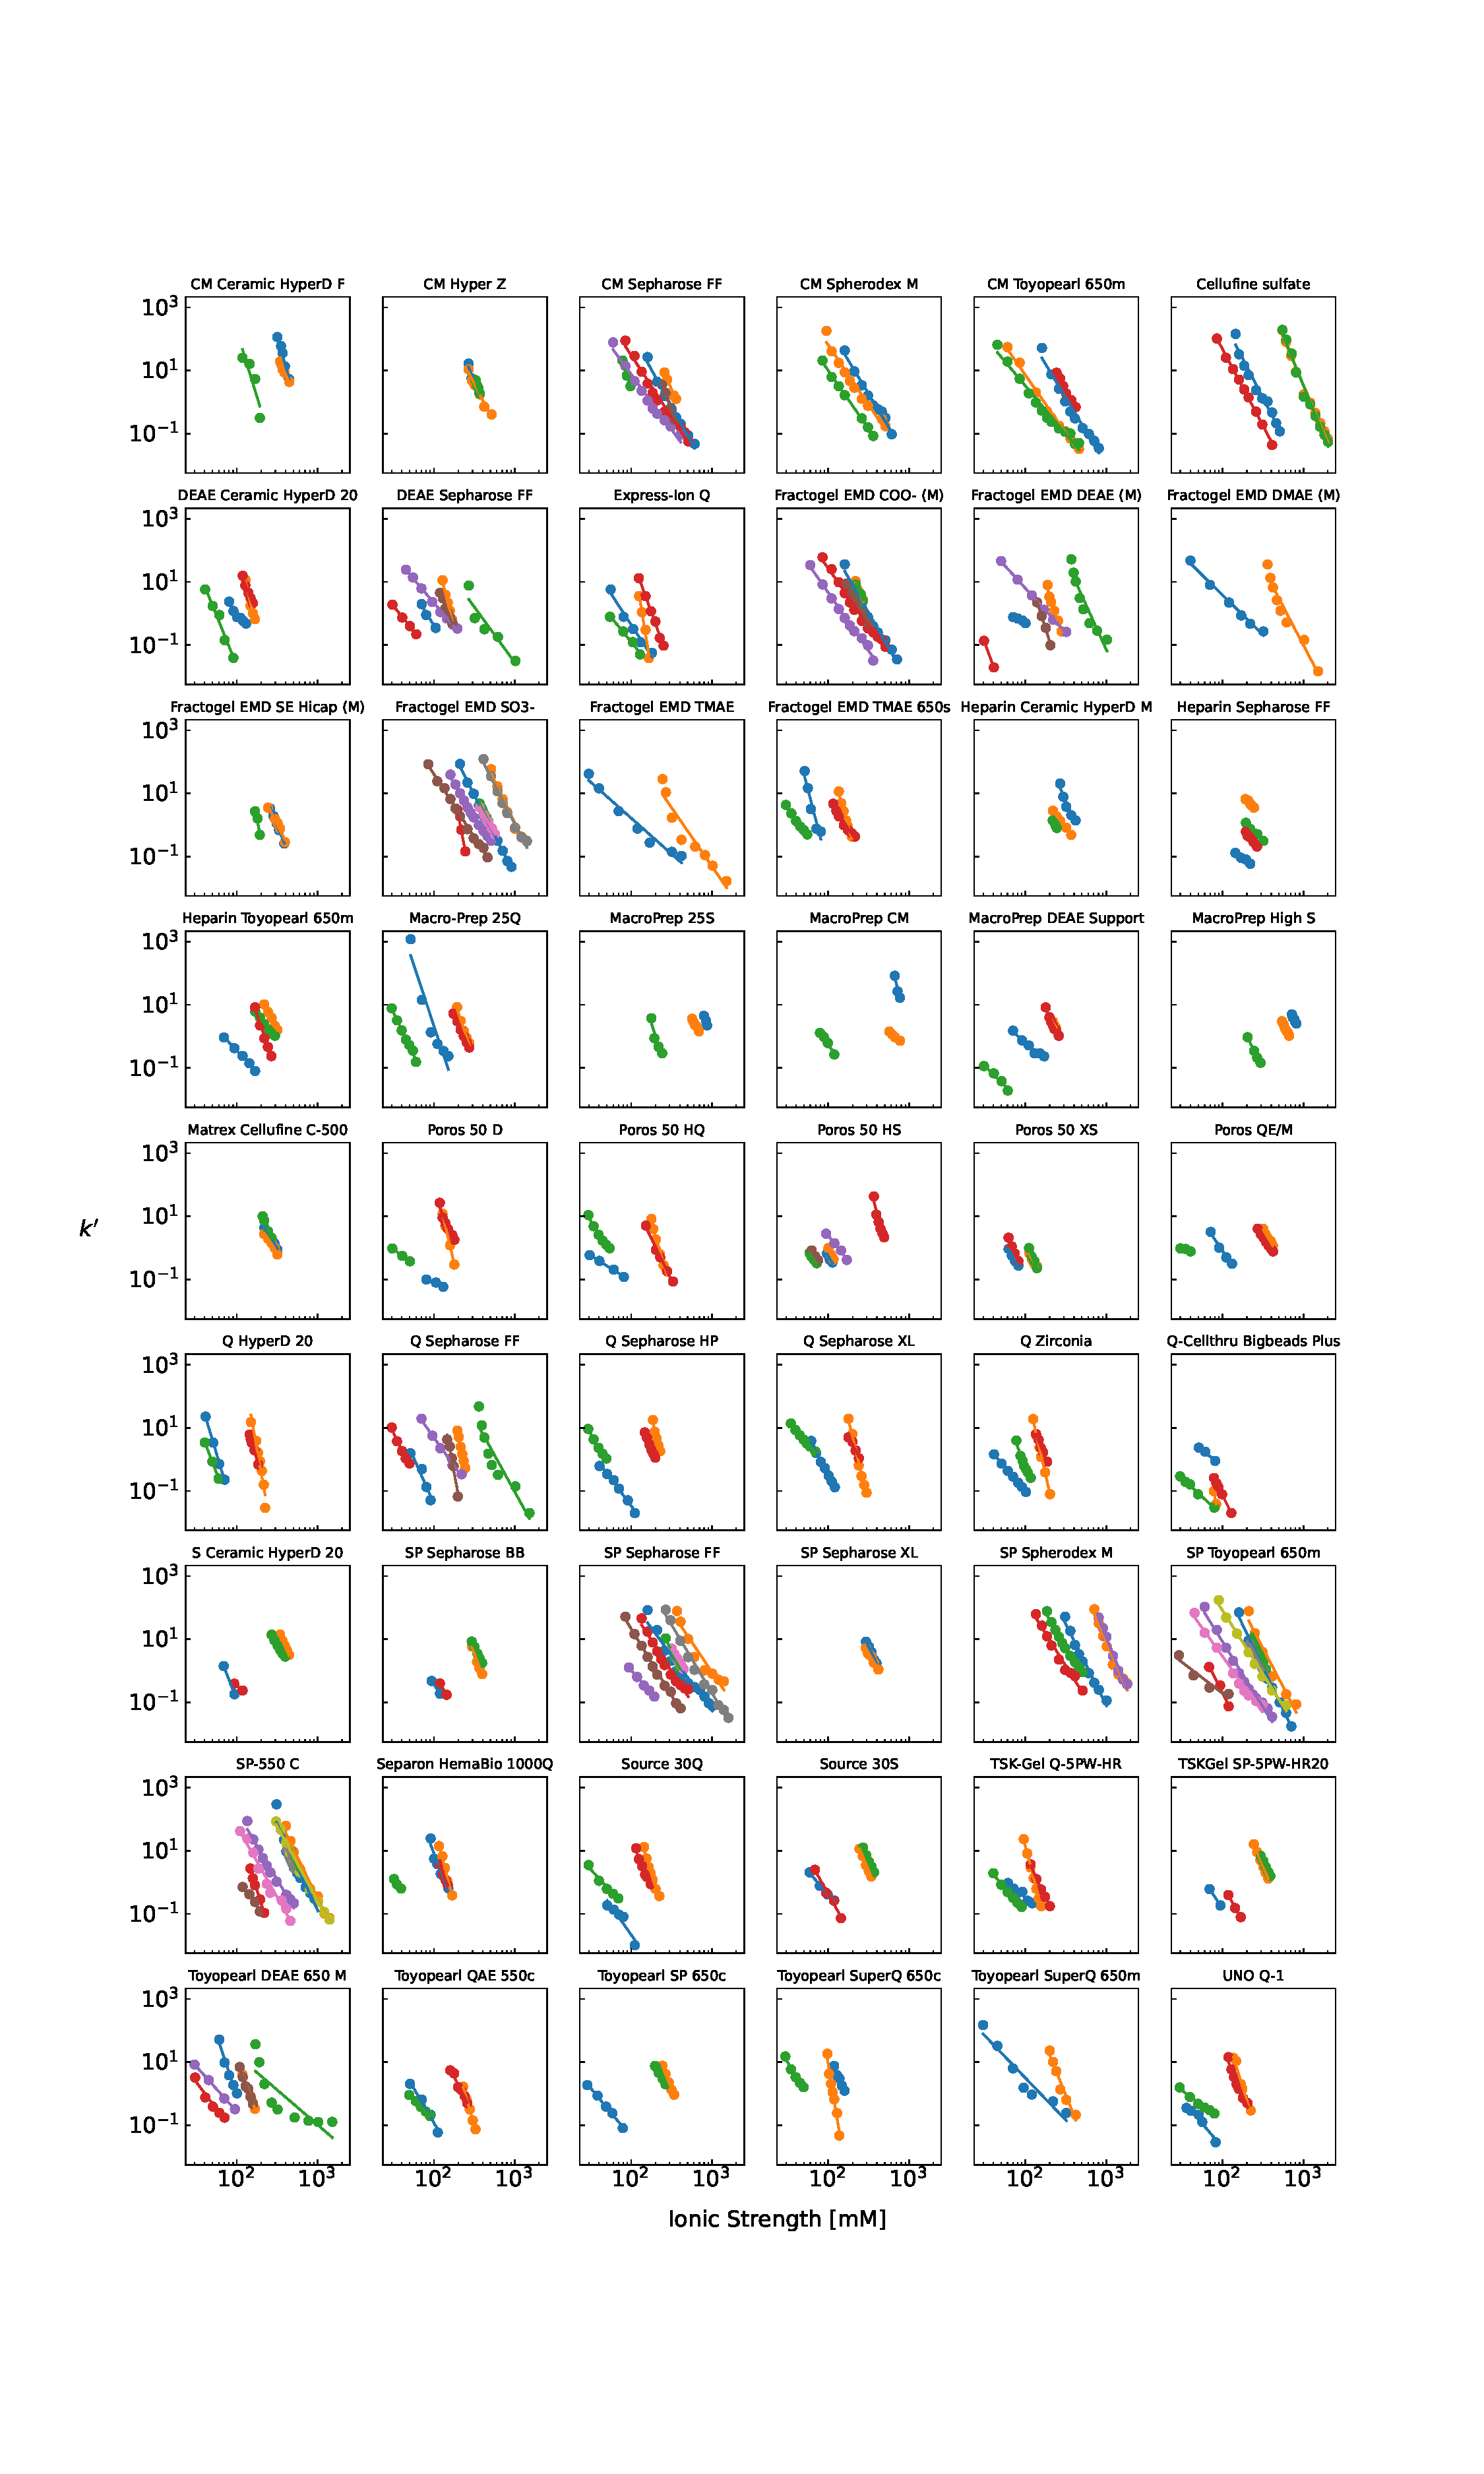
\includegraphics[width=1.15\textwidth]{figure_s2}\DIFaddendFL }
    \vspace{-4cm}
    \caption{Isocratic $k'$ data that were consolidated from the literature. Each series represents a unique protein-pH-resin combination, and lines represent quasi-SDM fits to the data. \DIFaddbeginFL \DIFaddFL{These data, which are available in the }\texttt{\DIFaddFL{Supplementary\_table\_S2.xlsx}} \DIFaddFL{file, were acquired by digitizing plots (using the Engauge Digitizer software), which may introduce some error into the precise $k'$ values.}\DIFaddendFL }

    \label{fig:consolidated data}
\end{figure}
\DIFaddbegin 


\begin{table}[h]
\caption{\DIFaddFL{Simulation parameters.}}
\label{tab:sim_params}
\begin{tabular}{l|l|l}
\DIFaddFL{Variable                                }& \DIFaddFL{Figures \ref{fig-fig:exploratory breakthrough curves},
                                                    \ref{fig-fig:initial breakthrough volumes vs Keq},
                                                    and \ref{fig:exploratory breakthrough curves - other concentrations}
                                        }& \DIFaddFL{Figure \ref{fig-fig:correlation of breakthrough volumes} }\\
\hline
\DIFaddFL{$L_{col}$ }{[}\DIFaddFL{cm}{]}                       & \DIFaddFL{4.2 }& \DIFaddFL{5.0 -- 20.0 }\\
\DIFaddFL{$r_p$ }{[}\DIFaddFL{$\mu$m}{]}                       & \DIFaddFL{25.0 }& \DIFaddFL{2.5 -- 100.0 }\\
\DIFaddFL{$\varepsilon_c$ }{[} \DIFaddFL{- }{]}                & \DIFaddFL{0.49 }& \DIFaddFL{0.49 }\\
\DIFaddFL{$\varepsilon_p$ }{[} \DIFaddFL{- }{]}                & \DIFaddFL{0.40 }& \DIFaddFL{0.40 }\\
\DIFaddFL{$u$, superficial velocity }{[}\DIFaddFL{cm/h}{]}     & \DIFaddFL{300 }& \DIFaddFL{100 -- 200 }\\
\DIFaddFL{$D_{ax}$ }{[}\DIFaddFL{m$^2$/s}{]}                   & \num{1.25e-7} & \DIFaddFL{Function of $u$}\\
\DIFaddFL{$k_{film}$ }{[}\DIFaddFL{m/s}{]}                     & \num{1.0e-3} & \num{1.0e-3} \\
\DIFaddFL{$D_p$ }{[}\DIFaddFL{m$^2$/s}{]}                      & \num{1.0e-11} & \num{5.0e-12} \DIFaddFL{-- }\num{4.0e-11}\\
\DIFaddFL{$a$ }{[}\DIFaddFL{m$^2$/s}{]} \DIFaddFL{(in $D_s = a K_{eq}^b$)  }& \num{7.76e-12} & \num{1.66e-12} \\
\DIFaddFL{$b$ }{[} \DIFaddFL{- }{]} \DIFaddFL{(in $D_s = a K_{eq}^b$)      }& \DIFaddFL{$-$1.54 }& \DIFaddFL{$-$0.24 }\\
\DIFaddFL{$K_{eq}$ }{[} \DIFaddFL{- }{]}                       & \num{1.0e0} \DIFaddFL{-- }\num{1.0e4} & \num{1.0e0} \DIFaddFL{-- }\num{1.0e4} \\
\DIFaddFL{$q_{max}$ }{[}\DIFaddFL{mg/ml column}{]}             & \DIFaddFL{100 }& \DIFaddFL{100 }\\
\DIFaddFL{$c_{load}$ }{[}\DIFaddFL{mg/ml}{]}                   & \num{1.0e-3} \DIFaddFL{-- }\num{1.0e1} & \num{1.0e-3}
\end{tabular}
\end{table}
\DIFaddend 

\end{document}
